\subsection*{Compressible Navier-Stokes}
\begin{frame}
    \begin{figure}[!htb]
      \begin{center}
        \subfigure{\label{fig:fob_uniform_2_sol}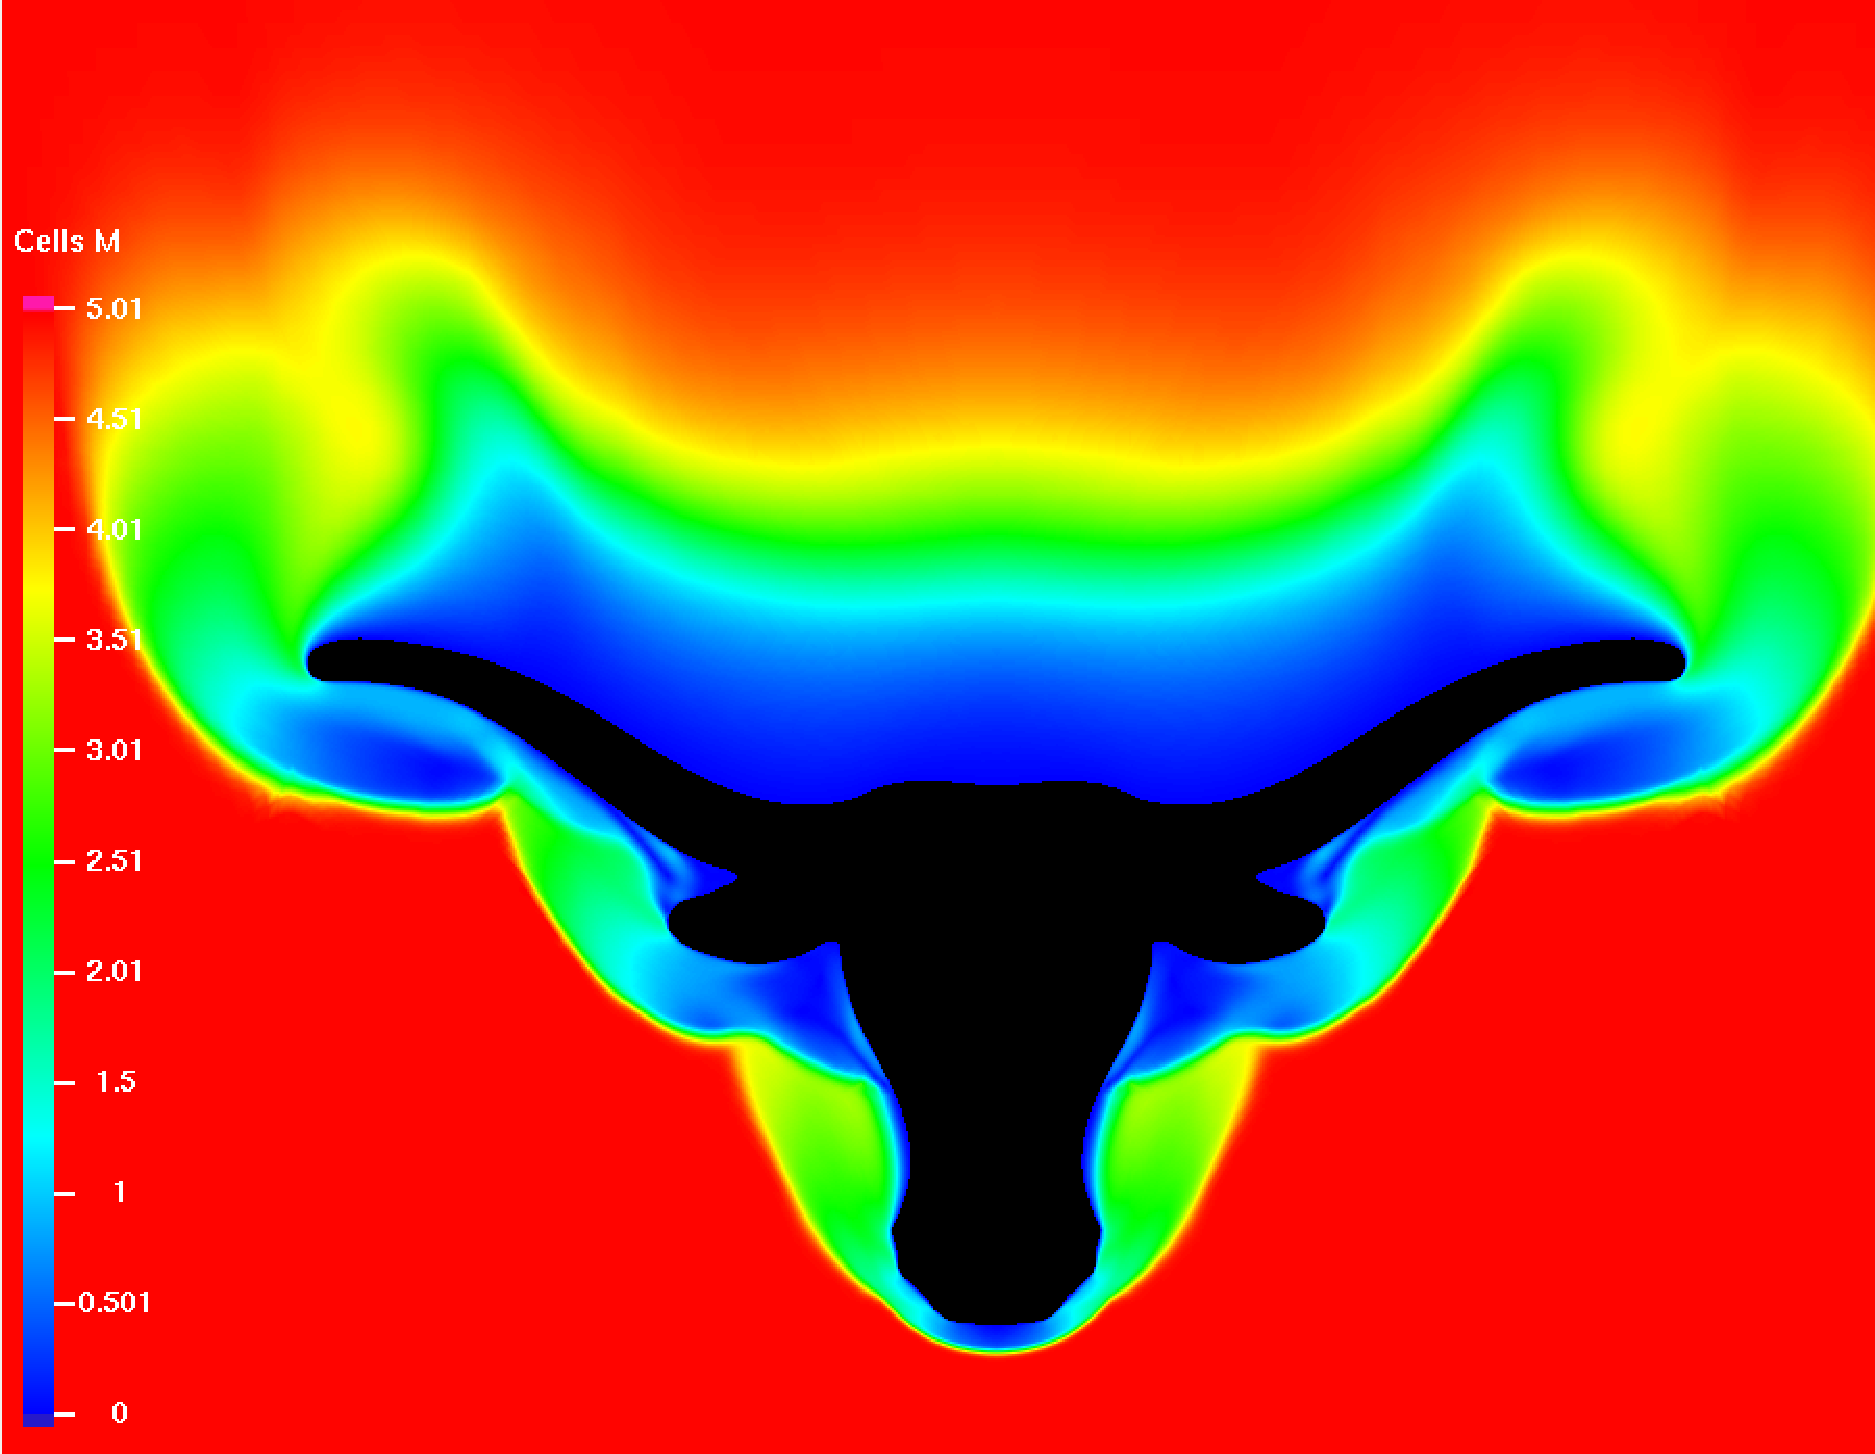
\includegraphics[width=.5\textwidth]{figures/Hypersonic_cow_mach}}
        %\subfigure{\label{fig:fob_adapt_3_sol}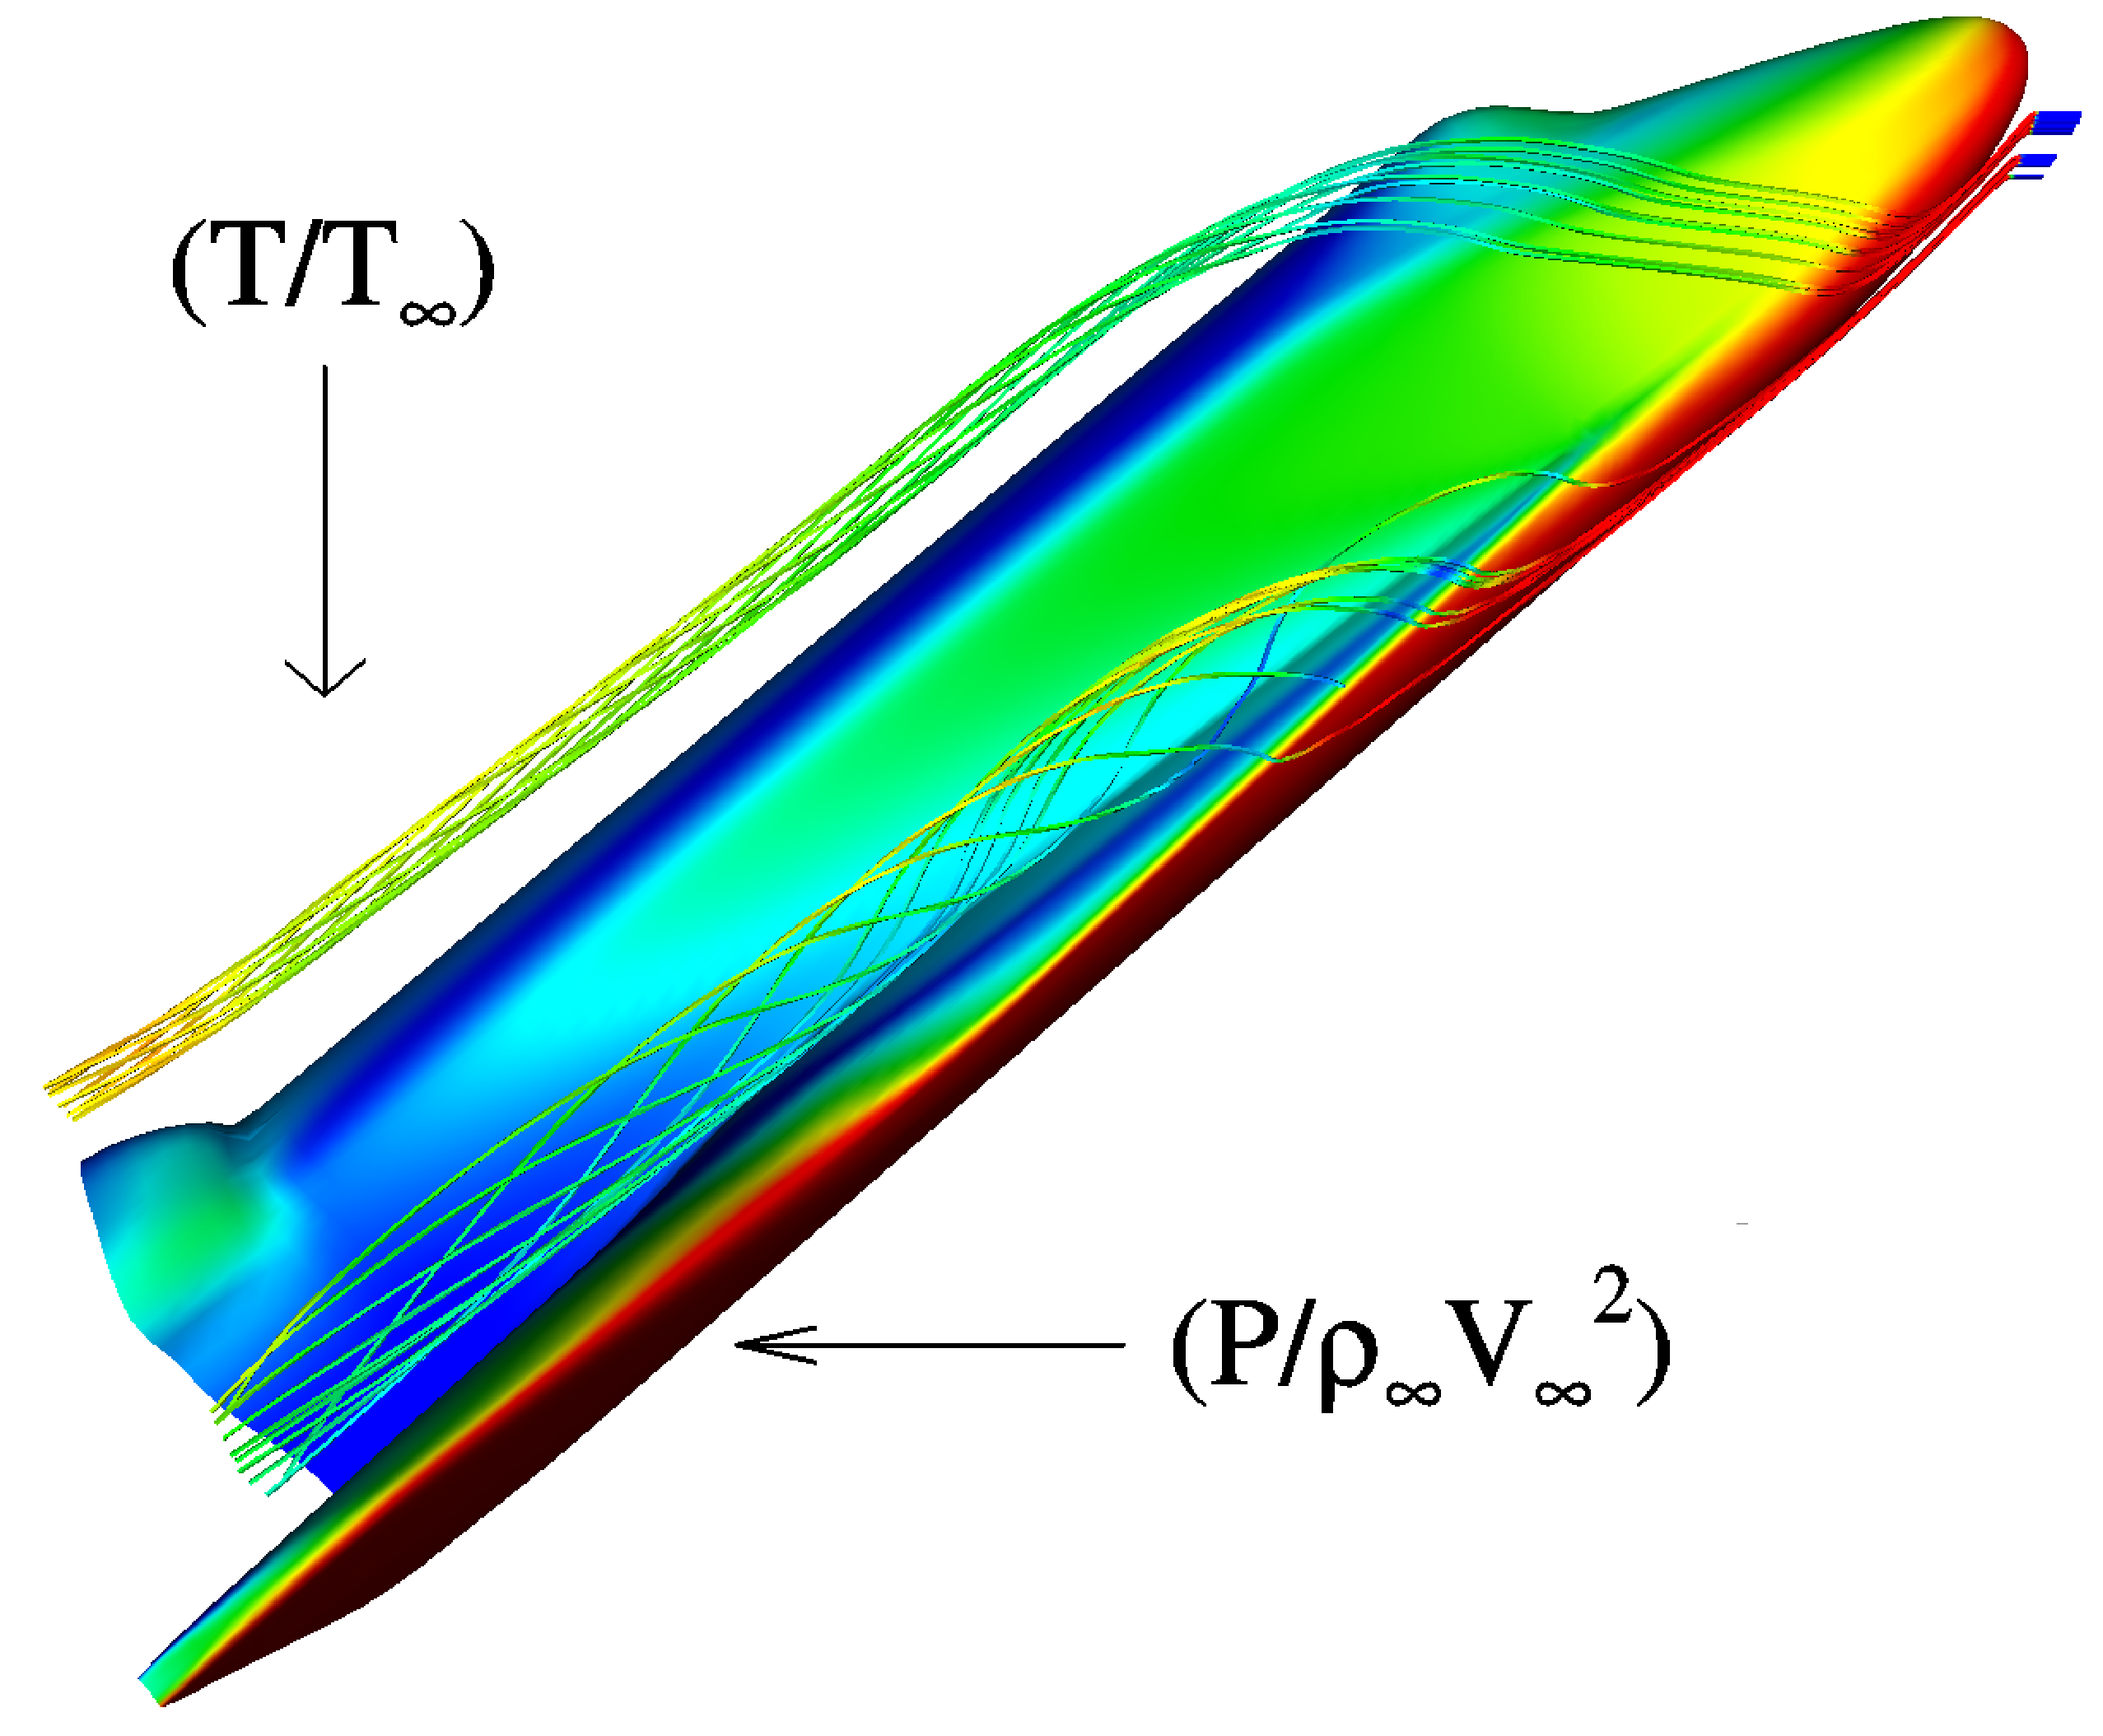
\includegraphics[width=.4\textwidth]{figures/Benkirk_orbiter_reentry_side_view}}
        \subfigure{\label{fig:fob_redist_adapt_10_sol}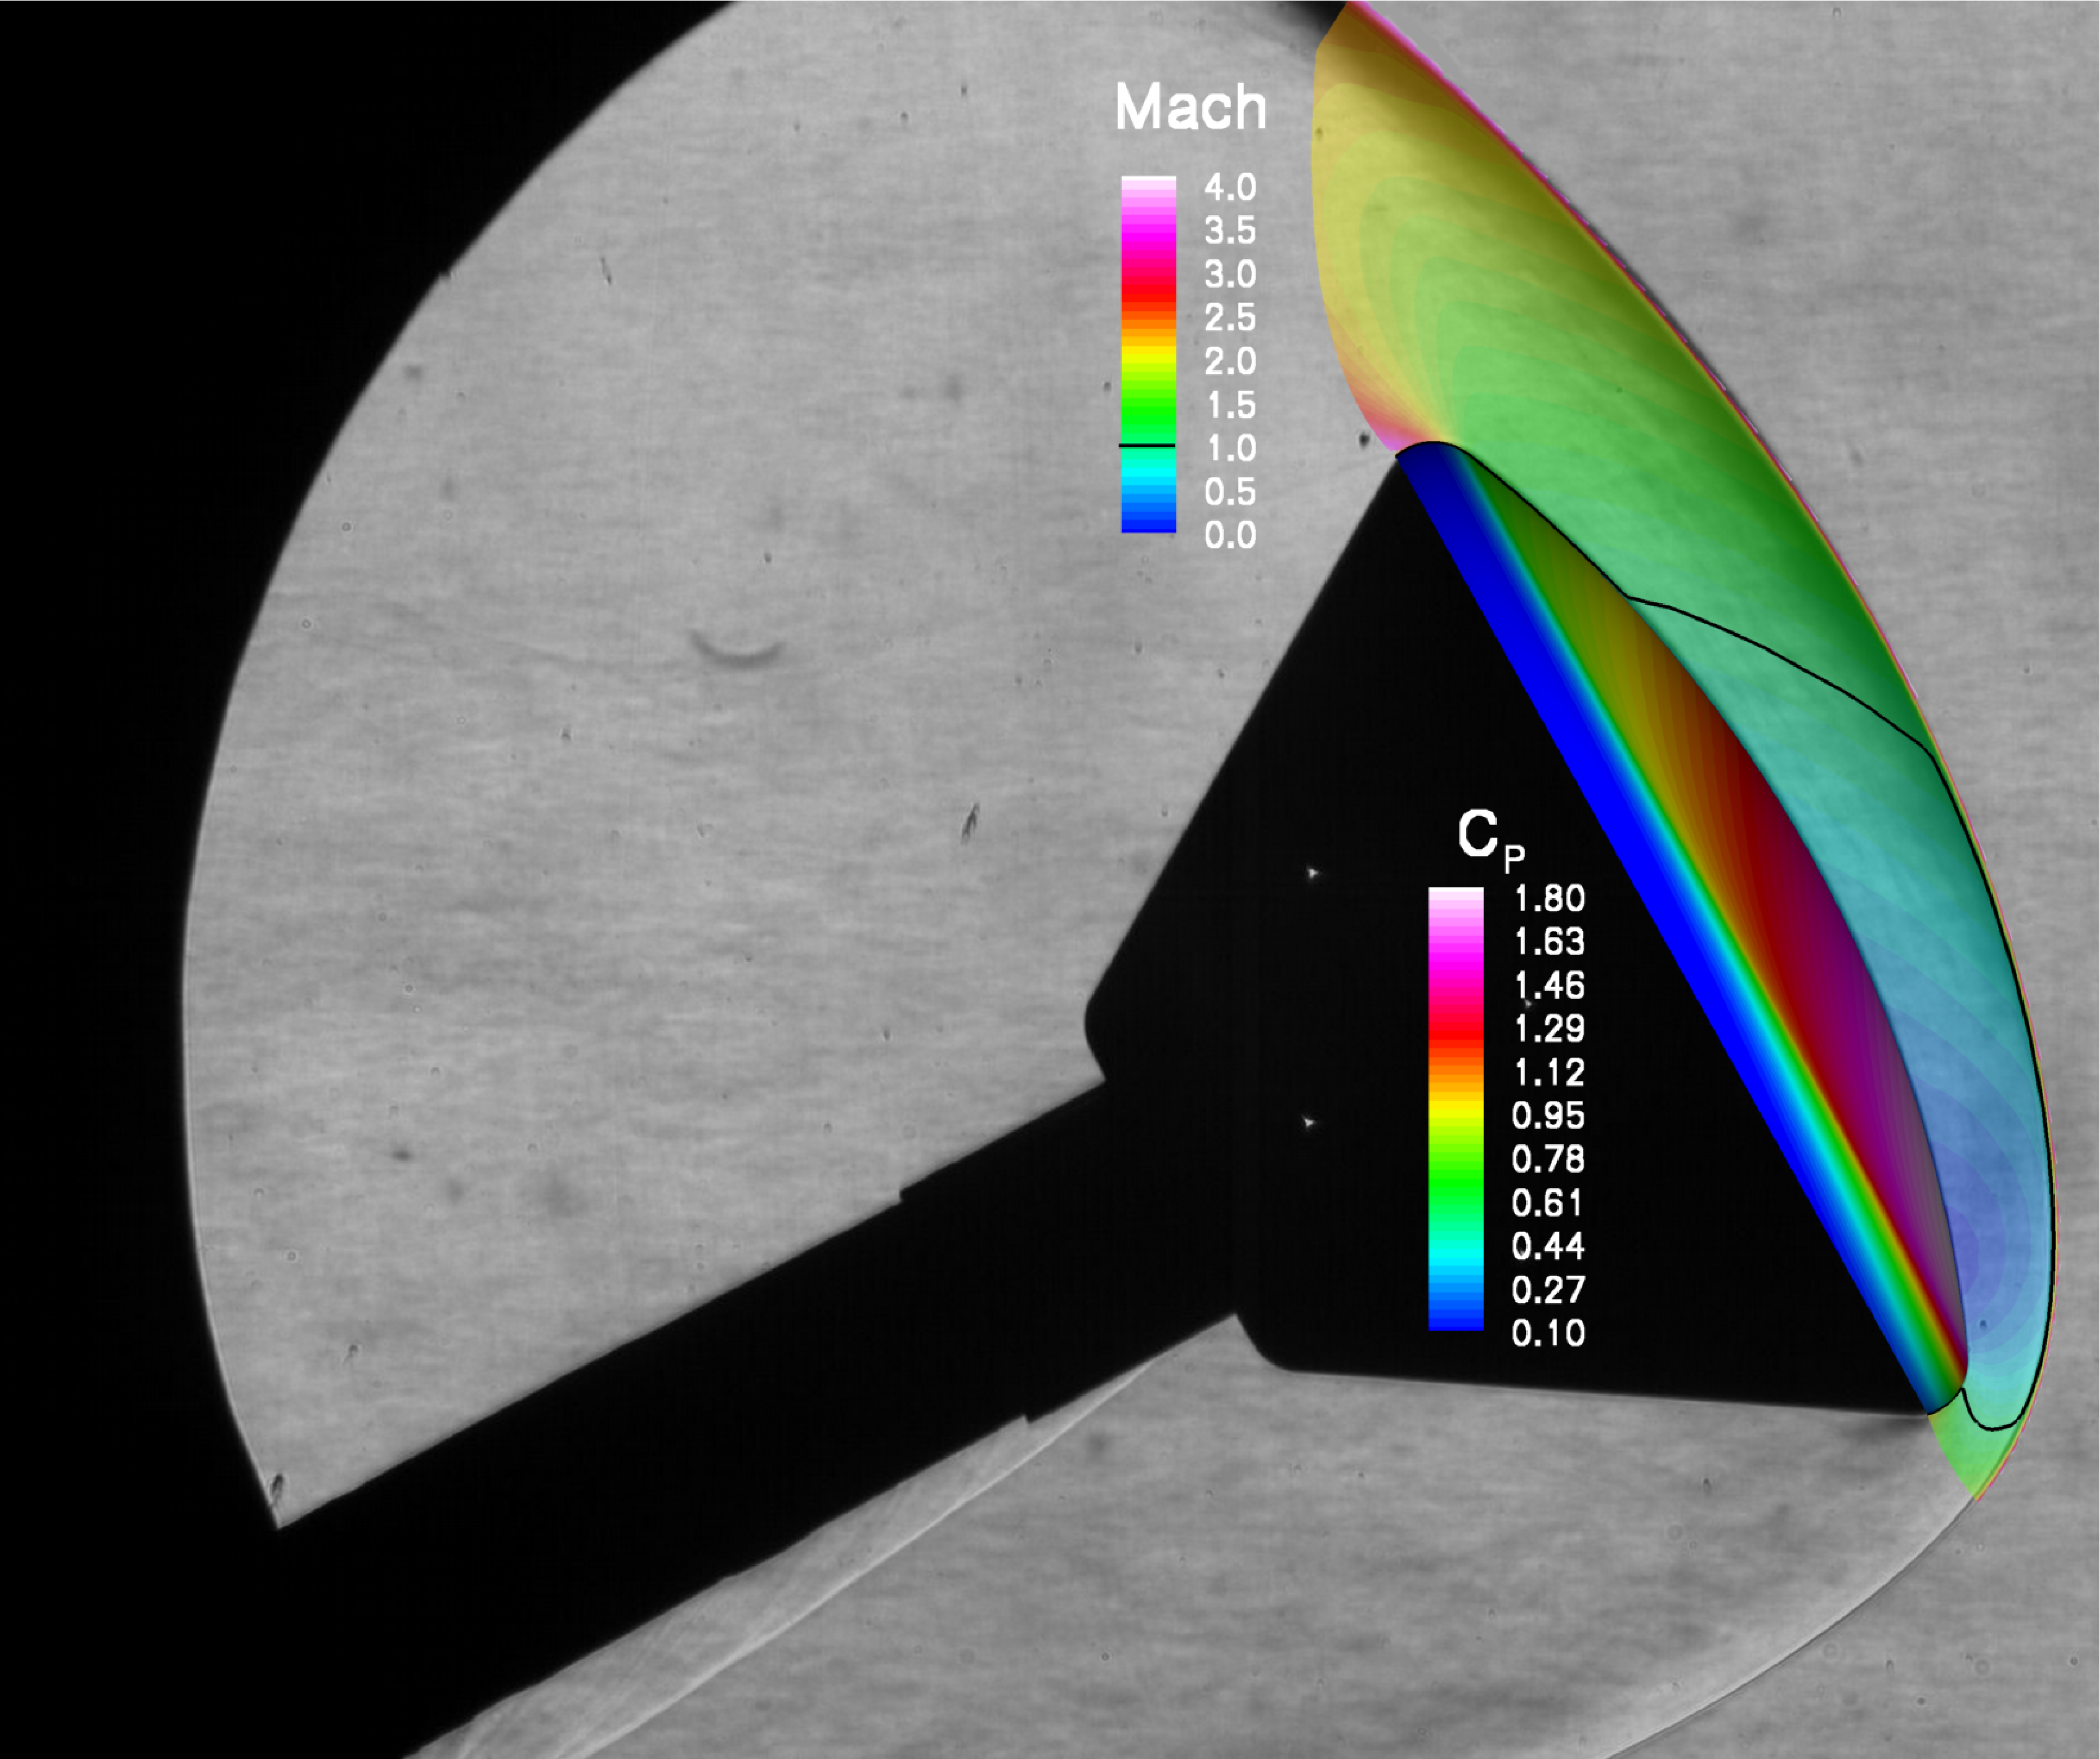
\includegraphics[width=.45\textwidth]{figures/Benkirk_schlieren}}
        %\subfigure{\label{fig:fob_redist_adapt_10_sol}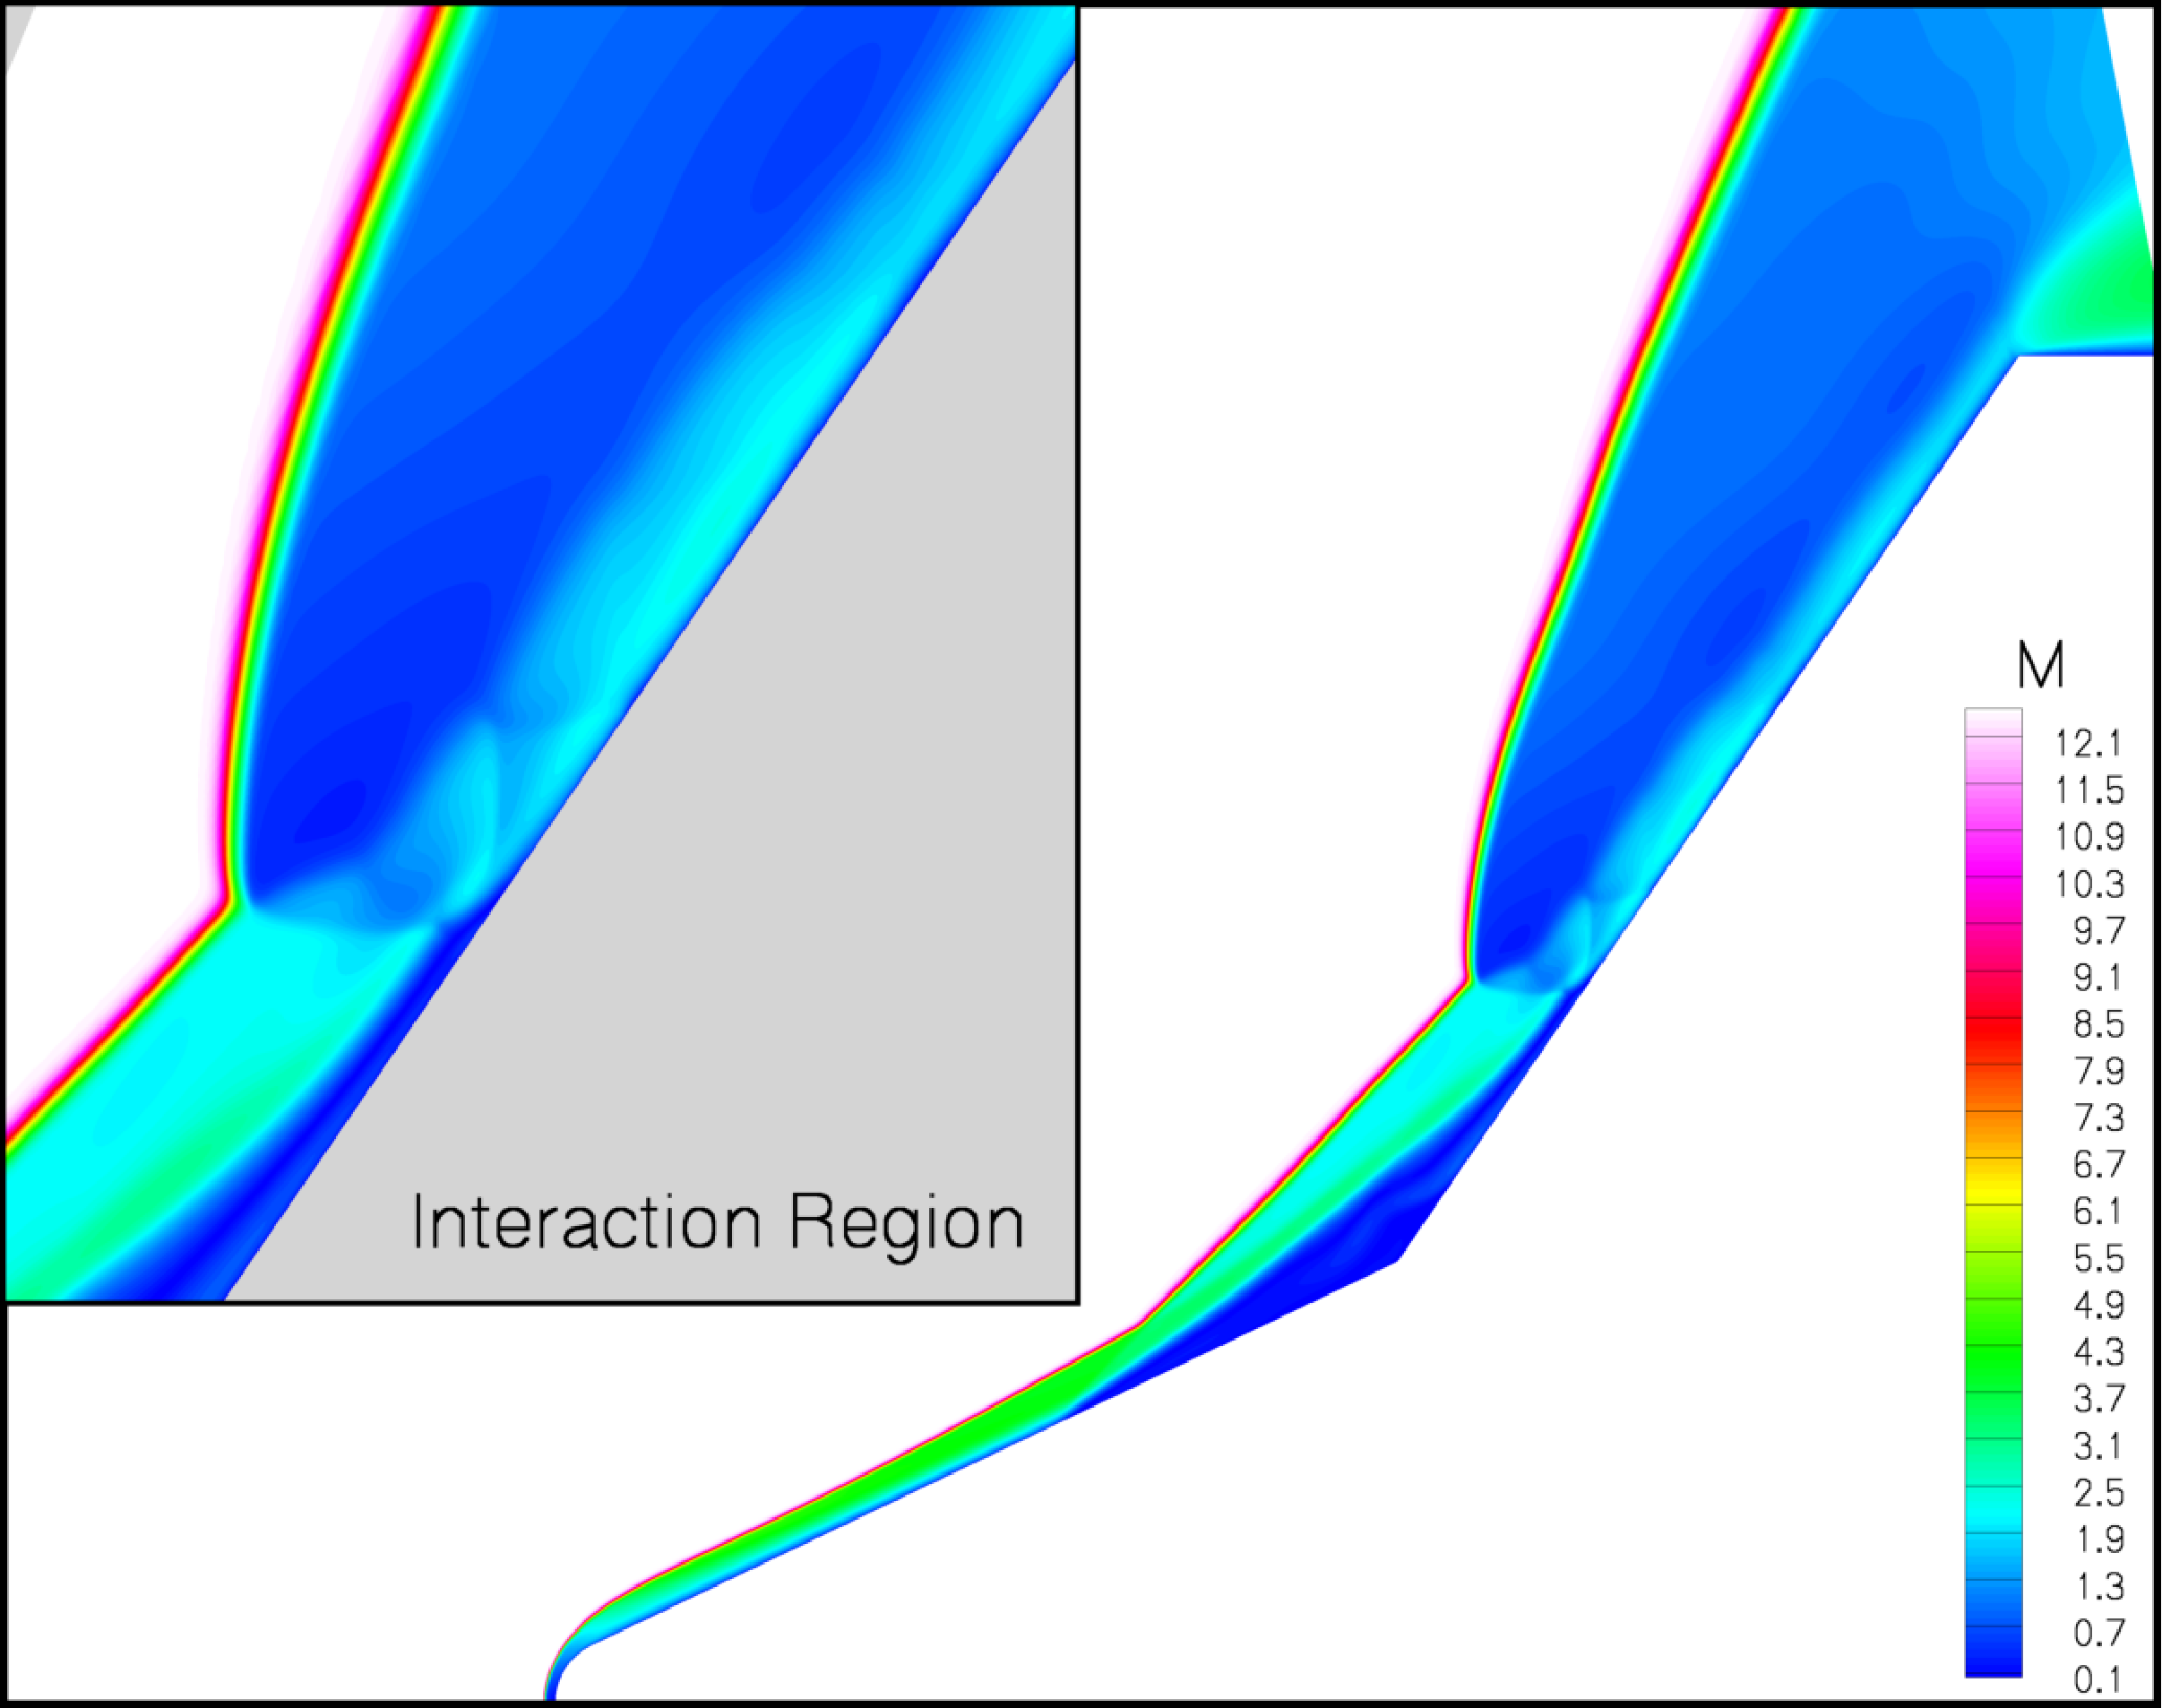
\includegraphics[width=.4\textwidth]{figures/Benkirk_double_cone_M}}
      \end{center}
    \end{figure}
\begin{itemize}
\item {LibMesh is being used in the development of the Orion CEV at NASA.}
\end{itemize}
\end{frame}


\subsection*{Surface-Tension-Driven Flow}
\begin{frame}%[t]
  \begin{center}
    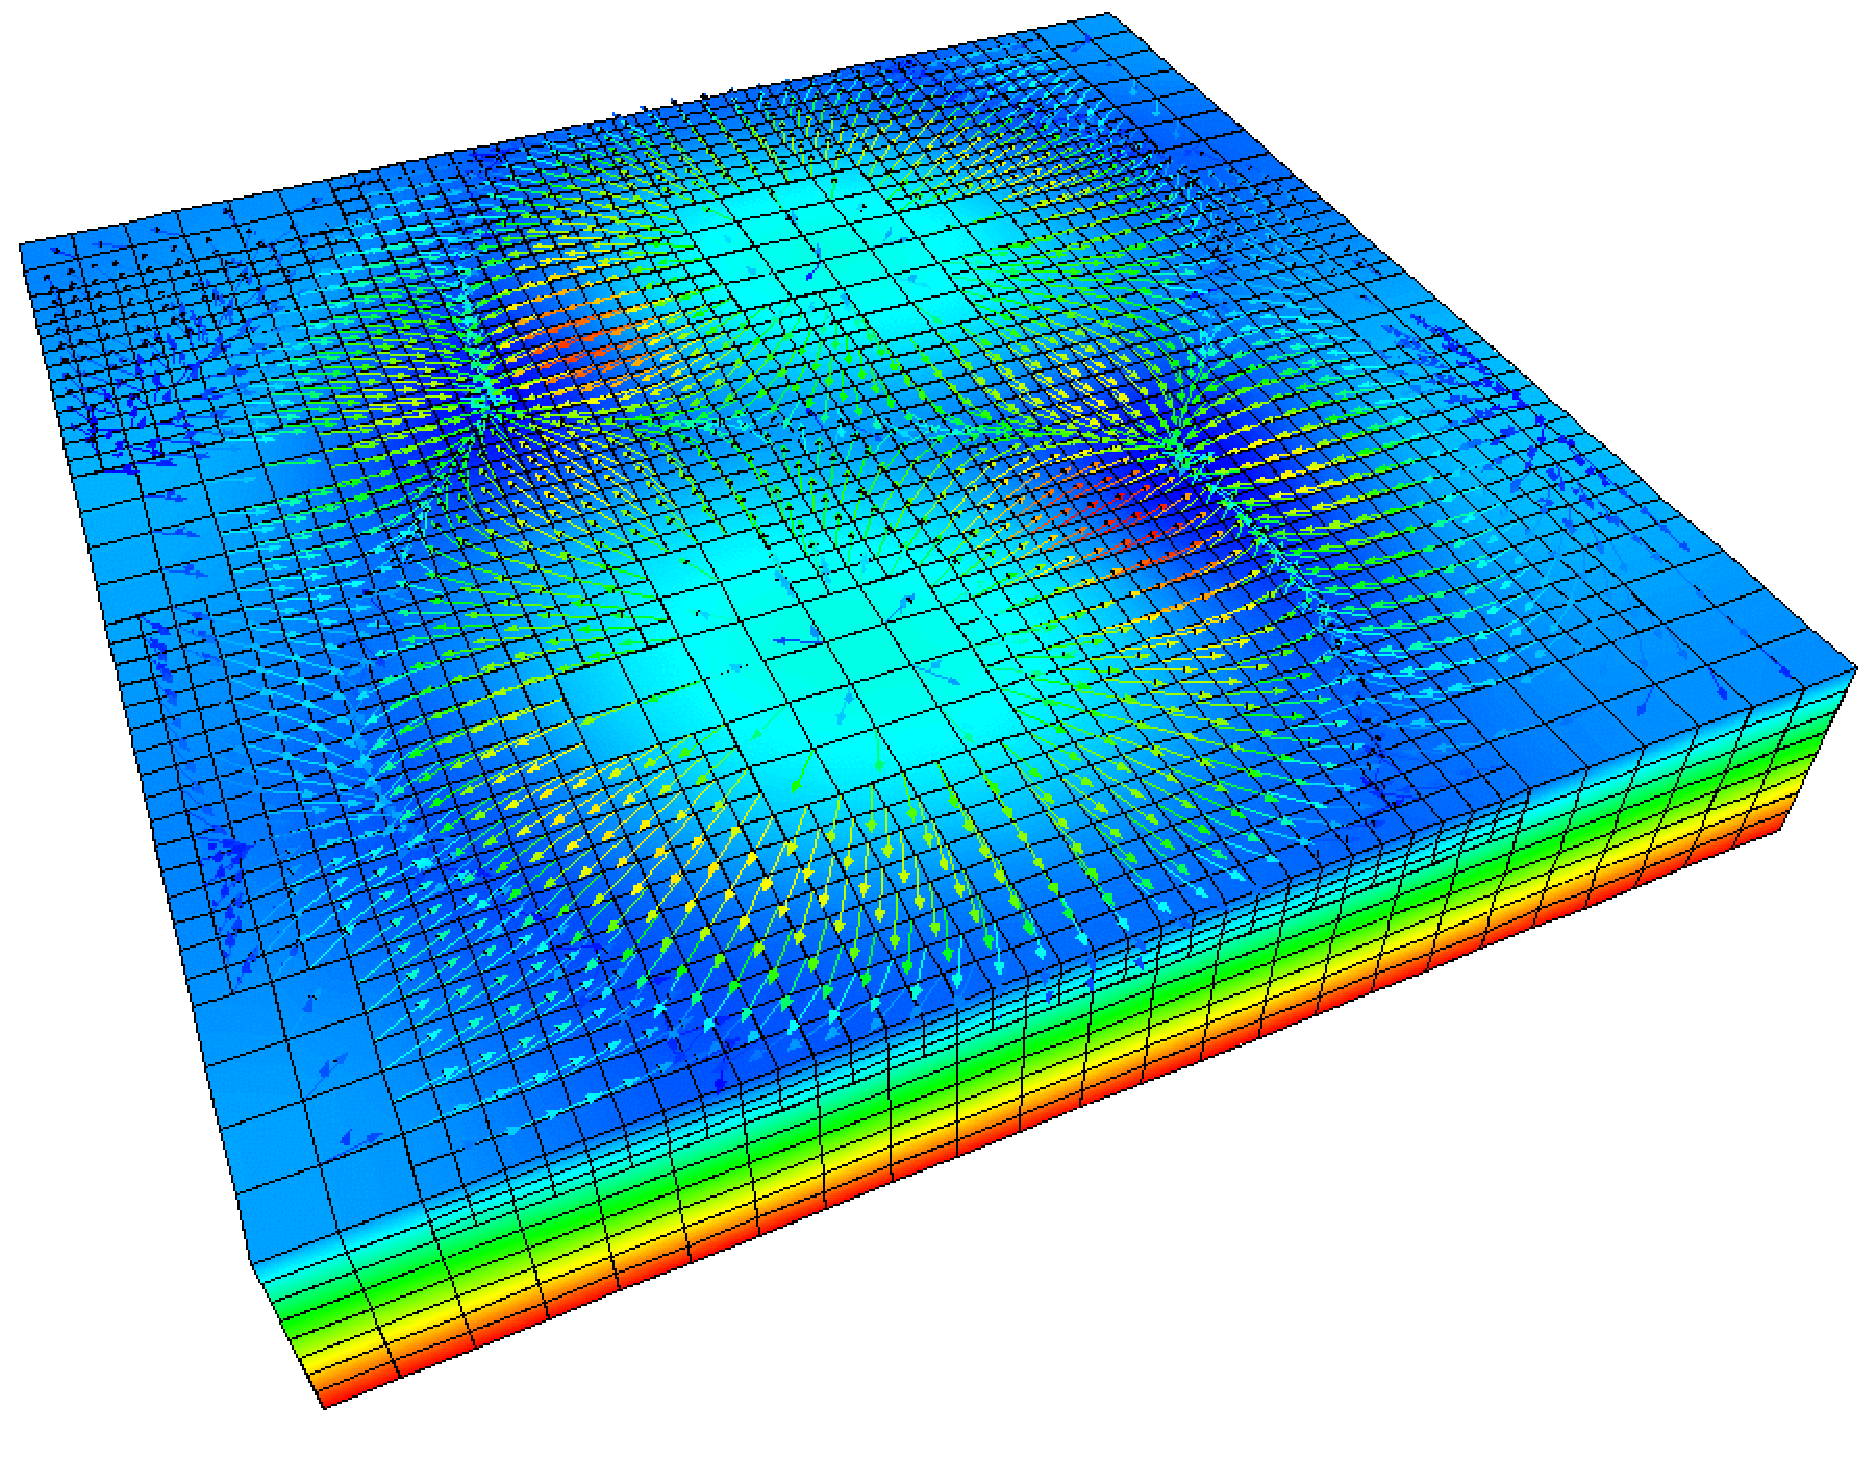
\includegraphics[width=.6\textwidth]{figures/rbm_adapt_soln}    
  \end{center}
  \vspace{-.25in}

%  \begin{block}{}
    \begin{itemize}
    \item{Adaptive grid solution shown
      with temperature contours and velocity vectors.      }
      \end{itemize}
%  \end{block}
\end{frame}


\subsection*{Tumor Angiogenesis}
\begin{frame}[t]
  \begin{center}
    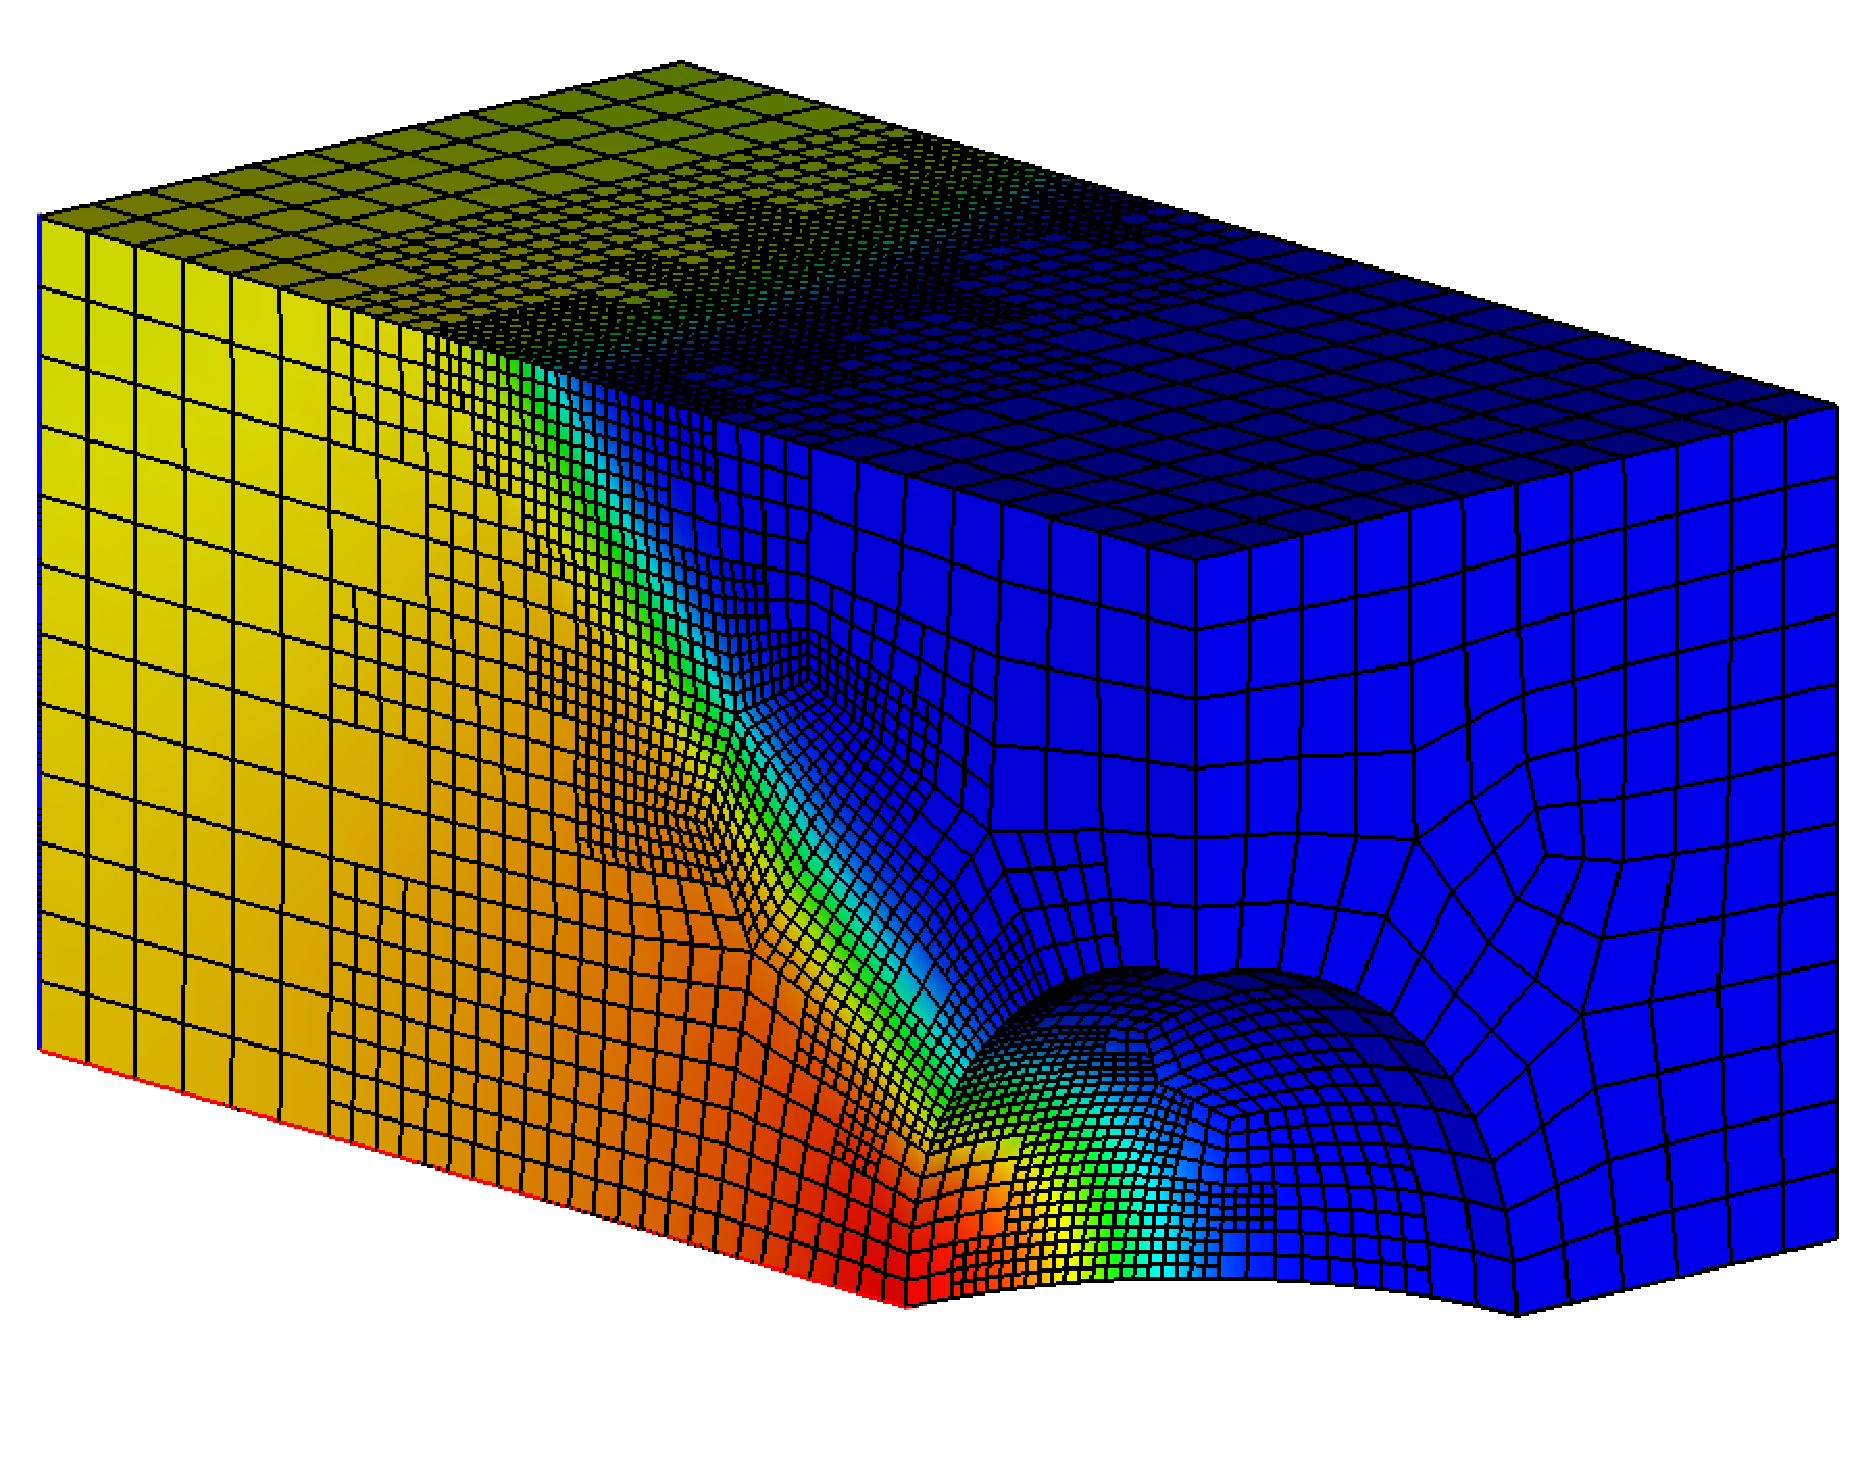
\includegraphics[width=.6\textwidth]{figures/tumor_model}    
  \end{center}
\vspace{-.35in}
%%   \begin{block}{}
    \begin{itemize}
    \item{A sharp advancing endothelial cell front approaches the
      tumor, eventually inducing blood vessel formation.      }
      \end{itemize}
%%   \end{block}
\end{frame}

\subsection*{Cahn-Hilliard Phase Separation}
\begin{frame}
\begin{center}
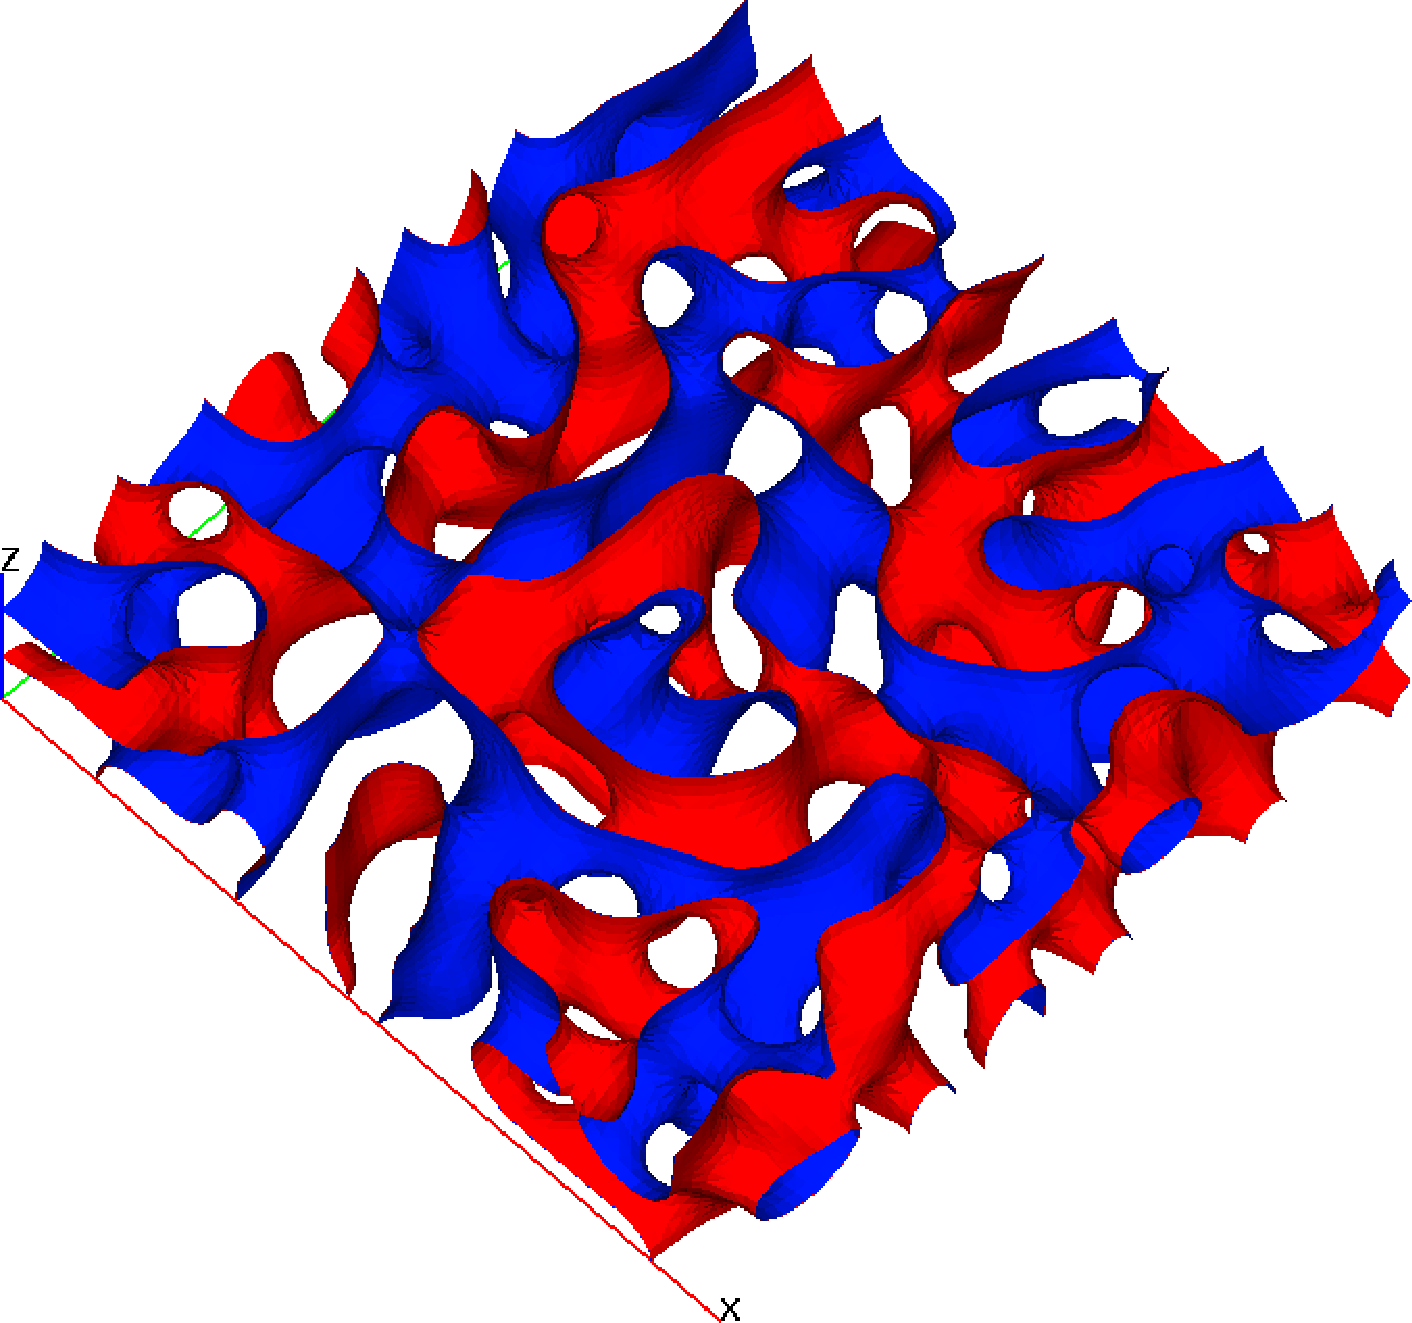
\includegraphics[width=.3\textwidth]{figures/ch3D02-048}
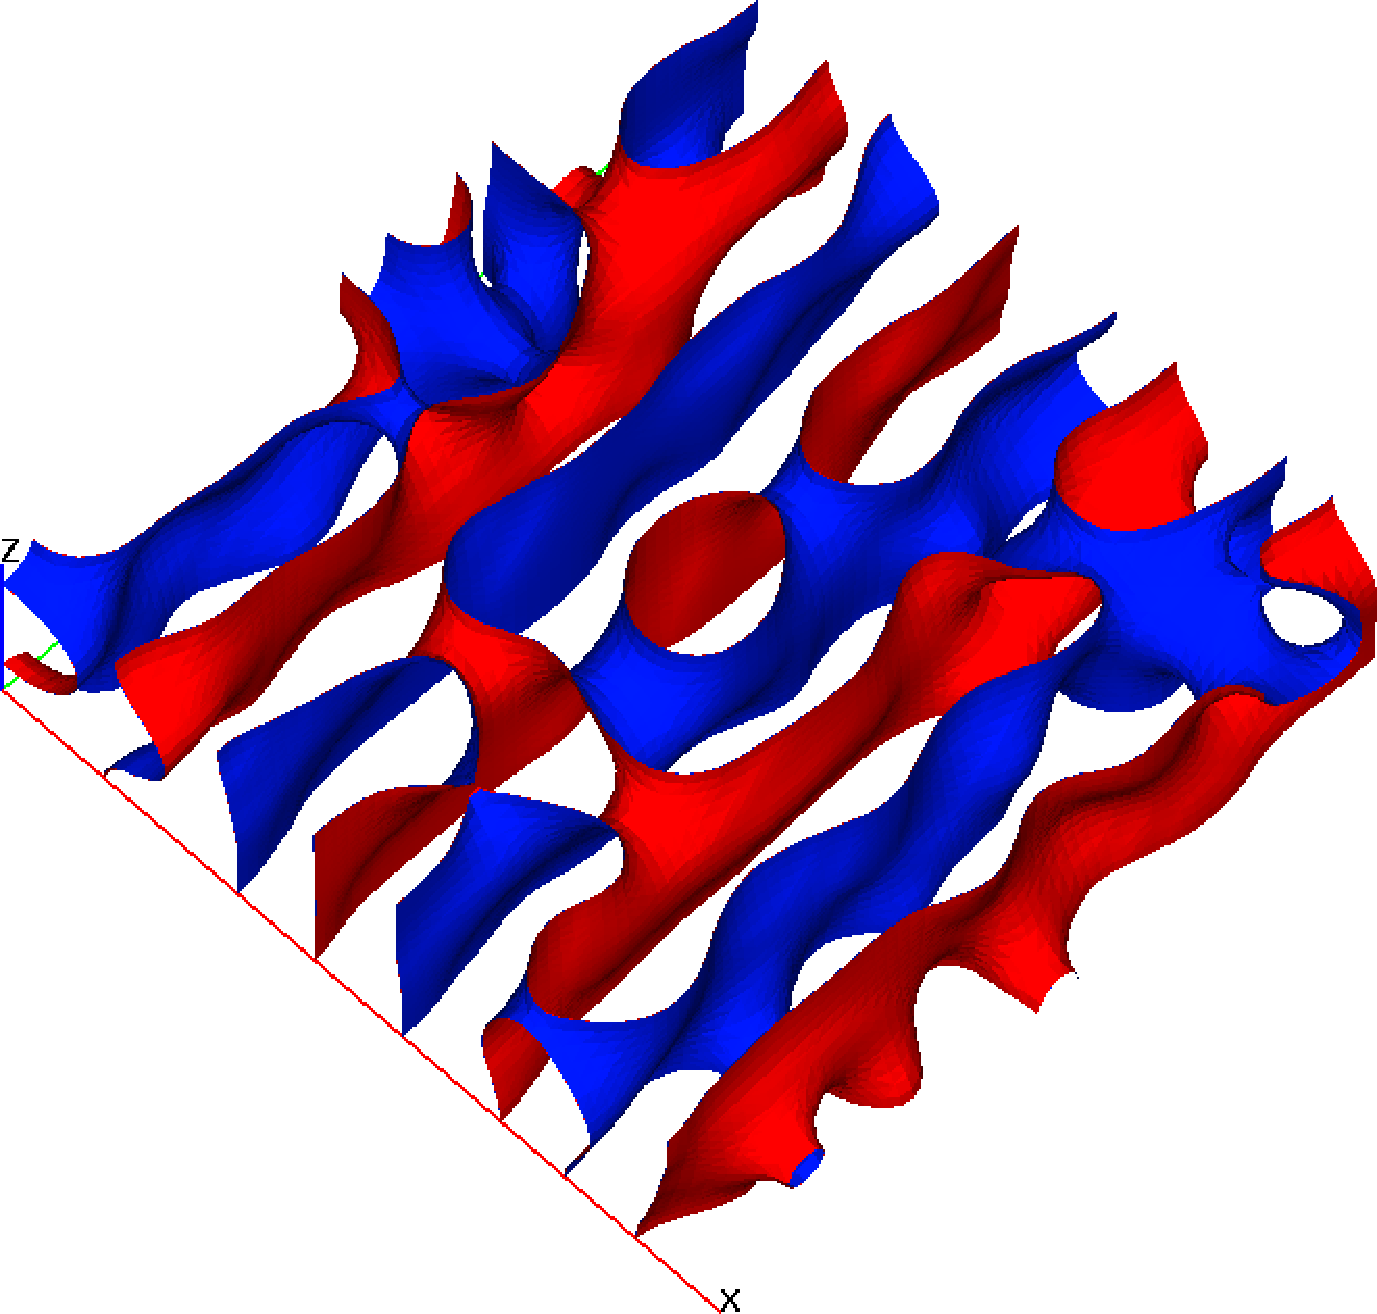
\includegraphics[width=.3\textwidth]{figures/ch3D02-096}
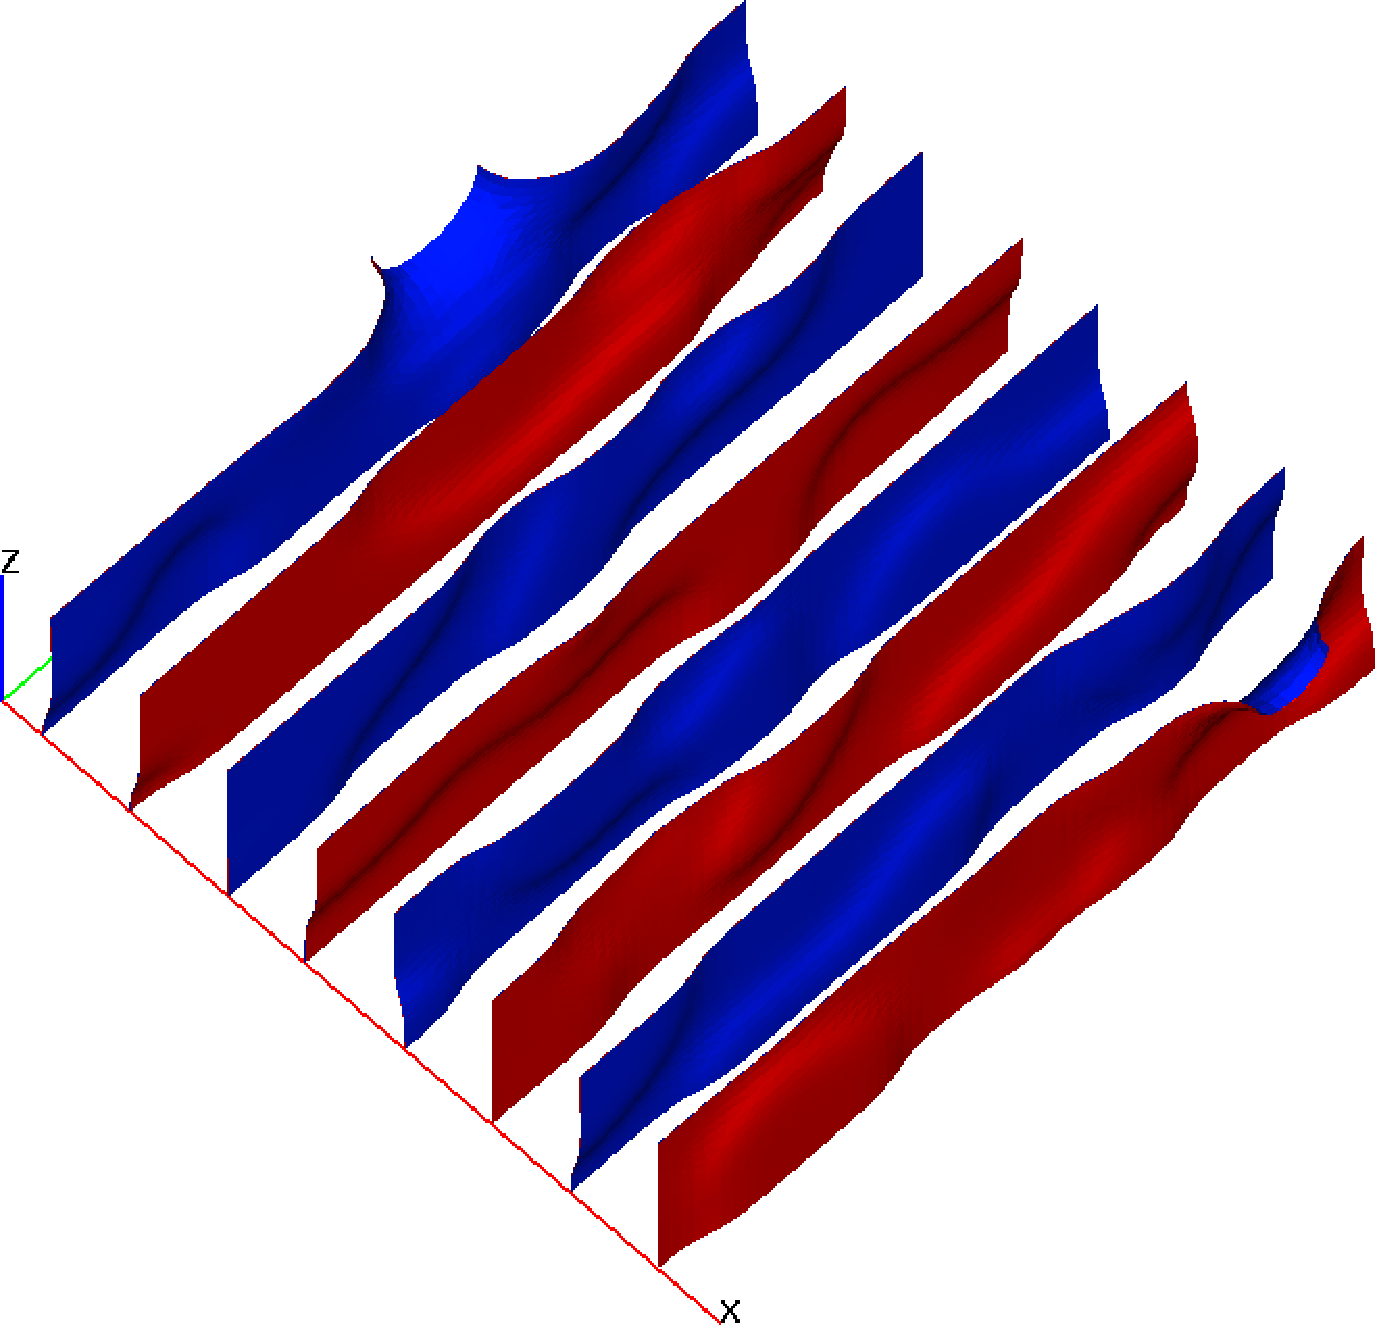
\includegraphics[width=.3\textwidth]{figures/ch3D02-192}
\end{center}
\begin{itemize}
\item Single-phase regions gradually coalesce
%\item Motion into curvature vector resembles surface tension
\item Patterning may occur when additional stresses are present
\end{itemize}
\end{frame}
